\begin{figure}[t]
  \centering
 \begin{subfigure}{0.95\textwidth}
    \begin{tabular}{ccccc}
      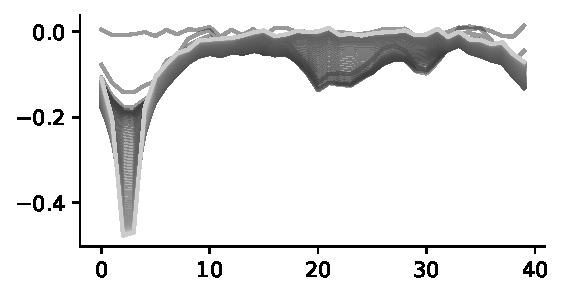
\includegraphics[width=0.25\linewidth]{figures/theory/rf_sim/ising_varphi.pdf} &
      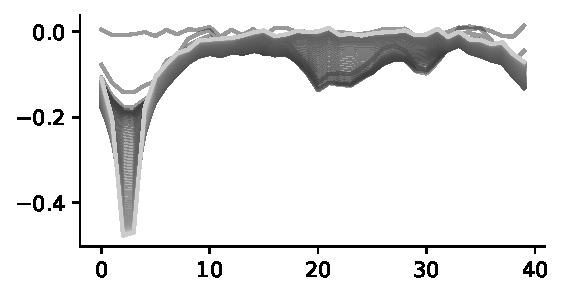
\includegraphics[width=0.25\linewidth]{figures/theory/rf_sim/ising_varphi.pdf} \\ 
      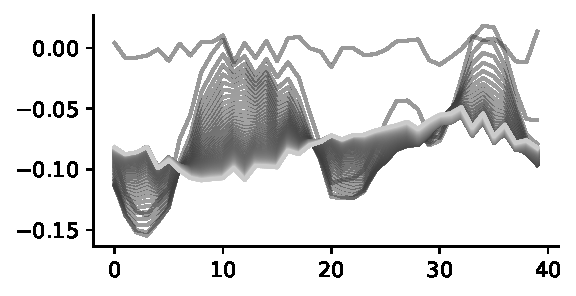
\includegraphics[width=0.25\linewidth]{figures/theory/rf_sim/gaussian_varphi.pdf} &
      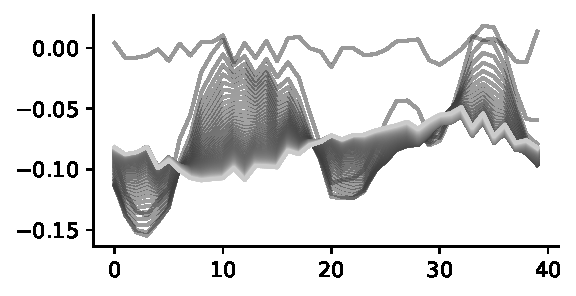
\includegraphics[width=0.25\linewidth]{figures/theory/rf_sim/gaussian_varphi.pdf} \\ 
      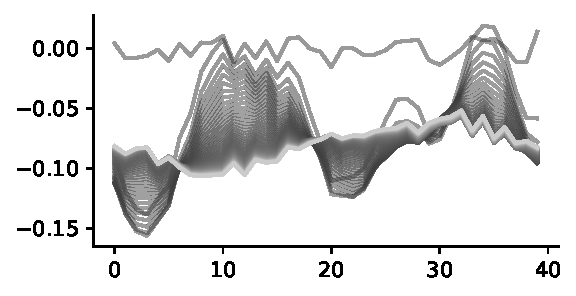
\includegraphics[width=0.25\linewidth]{figures/theory/rf_sim/alg5_varphi.pdf} &
      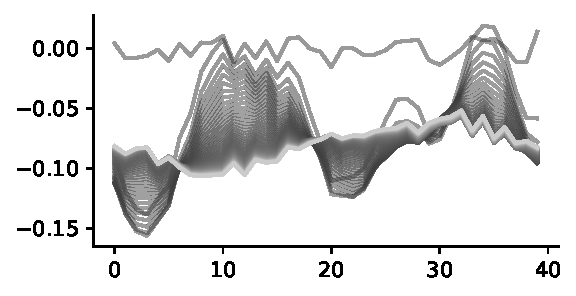
\includegraphics[width=0.25\linewidth]{figures/theory/rf_sim/alg5_varphi.pdf} \\ 
    \end{tabular}
  \end{subfigure}
  \caption{
    \nbr{Current figures are placeholders, from Fig. 3.}
    (\textbf{Left})
    \nb{Figure comparing empirical and analytical/approximated receptive fields}
    (\textbf{Right})
    \nb{Figure showing ICA components in 1D, 2D cases}
  }
  \label{fig:experiments}
\end{figure}
